\documentclass[french]{article}
\usepackage[T1]{fontenc}
\usepackage{fullpage}
\usepackage{babel}
\usepackage{hyperref}
\usepackage{graphicx}
\usepackage[justification=centering]{caption}
\usepackage{amsmath}
\usepackage{amssymb}
\usepackage{parskip}

\setlength{\parindent}{0pt}

\hypersetup{
  colorlinks=true,
  linkcolor=black,
  urlcolor=blue
}

\graphicspath{ {./img/} }
\title{%
    \huge Mathfinder  \\
    \bigskip
    \large E5 - Cas pratique \\ 
    Développeur en Intelligence Artificielle,
    titre professionnel enregistré au RNCP - École IA Microsoft by Simplon
    \vfill
    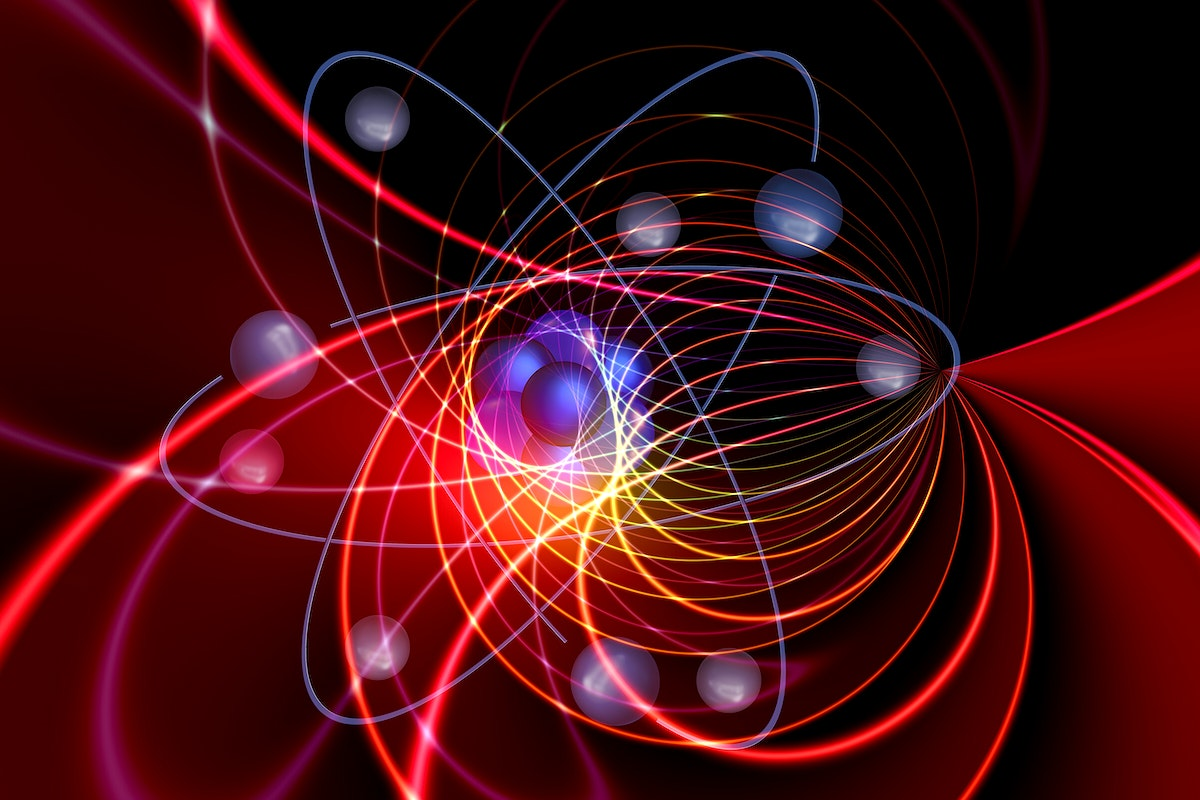
\includegraphics[width=14cm]{physics.jpg} % also works with logo.pdf
    \vfill}
\date{26 février 2024}
\author{par Vincent Papelard}

\begin{document}
    \renewcommand{\contentsname}{Table des Matières}
    \maketitle
    \pagenumbering{arabic}
    \pagenumbering{gobble}
    \newpage
    \tableofcontents
    \newpage
    \pagenumbering{arabic}

    \section{Contexte}
    Nous sommes les développeurs de Mathfinder, une application web à destination des physiciens. Mathfinder utilise une IA afin de calculer la fonction mathématique qui explique le mieux les données issues de leurs observations. L'application est destinée à être déployée directement sur les serveurs des établissements de recherche, qui réalisent les calculs.

    \begin{figure}[h]
        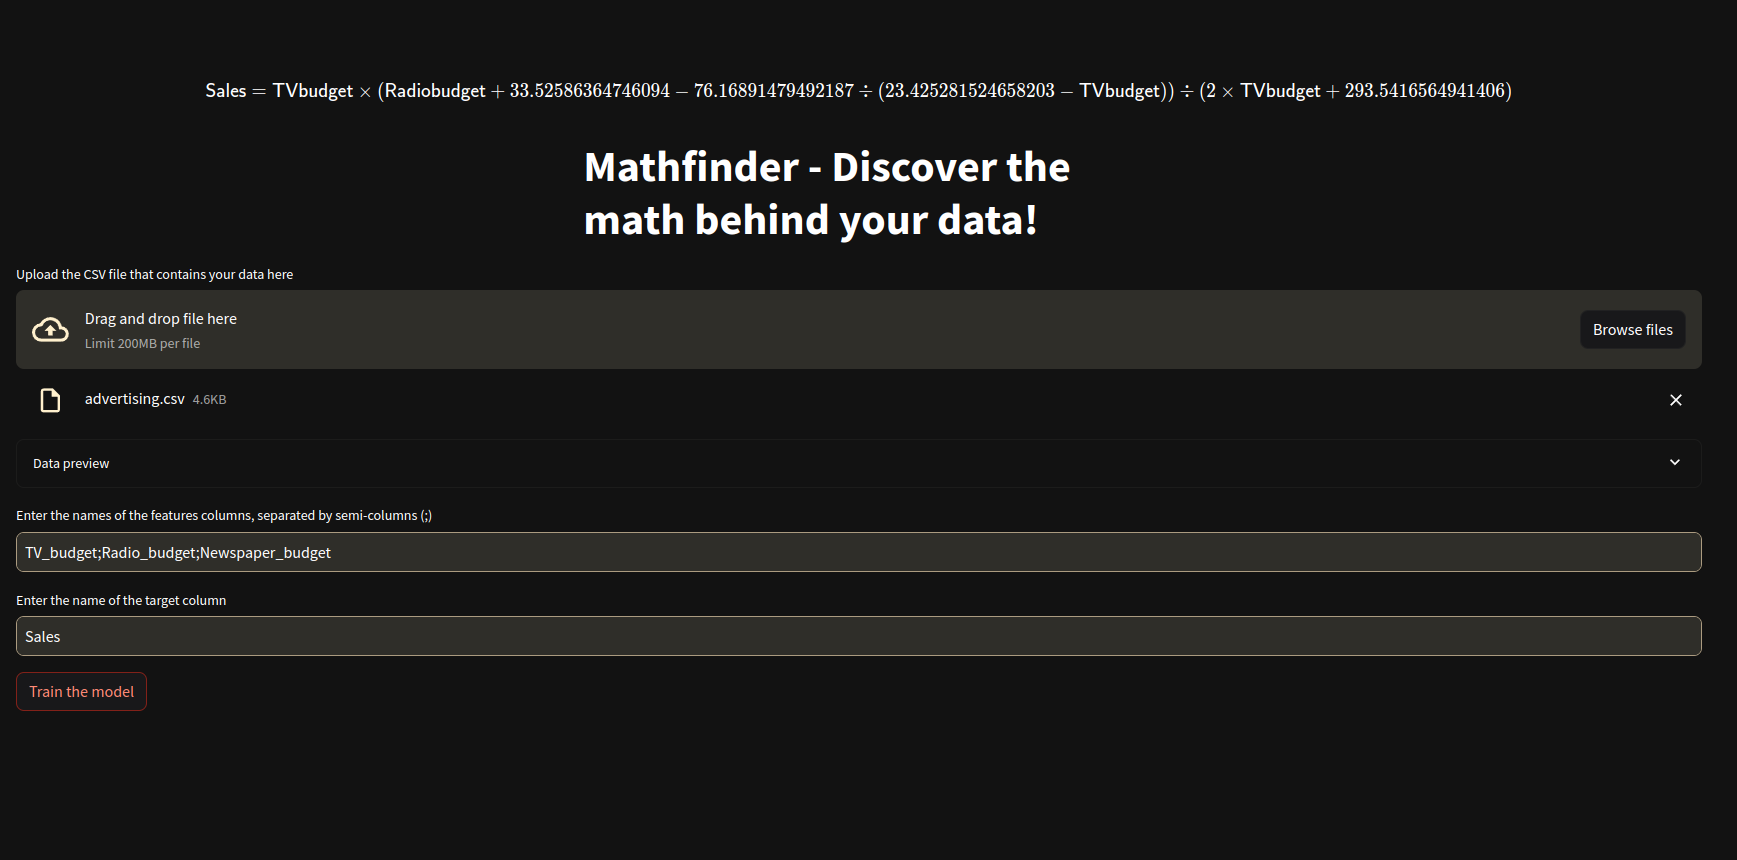
\includegraphics[width=12cm]{appli}
        \centering
        \caption{Mathfinder cherche une formule mathématique qui décrit les relations entre les données que l'on uploade. L'utilisateur peut entraîner un modèle sur ses propres données. Ce modèle est ensuite enregistré dans l'application et peut être réutilisé pour faire des prédictions}
        \centering
    \end{figure}

    Le directeur d'une grande université nous contacte. Les chercheurs de cette université ont récemment déployé Mathfinder sur leurs serveurs, mais ils rencontrent des bugs. Insatisfait de notre outil, le directeur exige que nous corrigions ces bugs et nous envoie un descriptif de tous les problèmes rencontrés :
    \begin{itemize}
        \item L'application crash quand on essaie de lui faire prédire les valeurs de deux colonnes ou plus
        \item L'application crash si on ne sépare pas le nom de chaque colonne avec des points-virgules sans espace avant ou après
        \item L'application crash s'il manque des valeurs dans certaines colonnes dans le fichier CSV fourni.
    \end{itemize}
    Par ailleurs, plusieurs chercheurs de son établissement ont rencontré un problème étrange : la précision de leurs modèles d'IA se dégrade avec le temps ! Perplexe, le directeur se tourne vers nous pour que nous réglions ce problème.

    Ce dossier comporte deux volets :
    \begin{itemize}
        \item Le débugging des problèmes rencontrés, de la reproduction du bug à sa résolution
        \item La mise en place de mécanismes de surveillance des modèles et d'alerte.
    \end{itemize}
    Le code associé à ce projet est disponible \href{https://github.com/vinpap/mathfinder}{sur GitHub}.

    \section{Traitement des problèmes techniques}
    \subsection{Méthodologie de debugging}
    La résolution des bugs est divisée en plusieurs étapes :
    \begin{itemize}
        \item Reproduction du bug
        \item Écriture d'un test unitaire qui reproduit le bug
        \item Recherche de la source du problème
        \item Correction du bug
    \end{itemize}
    \textbf{GitHub} est un outil crucial durant ce processus. Deux fonctionnalités de la plateforme sont notamment exploitées ici :
    \begin{itemize}
        \item Les tickets GitHub nous permettent de documenter le debugging en enregistrant une trace des actions prises pour corriger chaque bug
        \item Afin de ne pas compromettre le fonctionnement de l'application, le debugging de chaque problème est réalisé sur une branche qui lui est propre. Lorsque le problème est réglé, cete branche est fusionnée à la branche principale de l'application à l'aide d'une pull request.
    \end{itemize}
    \subsection{Résolution des problèmes}
    \textbf{Problème 1 : L'application crash quand on essaie de lui faire prédire les valeurs de deux colonnes ou plus (\href{https://github.com/vinpap/mathfinder/issues/2}{lien vers le ticket})}

    Si un utilisateur tente d'entraîner son modèle en spécifiant plus de deux valeurs cibles, l'application crash avec une exception ValueError. Un utilisateur mentionne avoir reçu le message \textit{"y should be a 1d array, got an array of shape (200, 2) instead"}.

    Ce problème est lié à une limitation du modèle de régression utilisé par Mathfinder : il ne peut générer qu'une seule valeur cible. Cette contrainte n'apparaît nul part sur l'interface cependant, et l'application permet malgré tout à l'utilisateur d'entrer plusieurs noms de colonne dans le formulaire. Deux mesures ont été mises en place pour régler ce bug :
    \begin{itemize}
        \item Le code Python a été modifié pour détecter l'apparition d'une exception ValueError. Si le format des données en entrée du modèle contient plus d'une dimension, on afiche alors un message d'erreur pour demander à l'utilisateur de n'entrer qu'un seul nom de colonne.
        \item Le texte de l'interface a été mis à jour pour demander à l'utilisateur d'entrer UN nom de colonne.
    \end{itemize}

    \textbf{Problème 2 : L'application crash si on laisse des espaces avant ou après les points-virgules qui séparent les noms des colonnes (\href{https://github.com/vinpap/mathfinder/issues/3}{lien vers le ticket})}

    L'application demande aux utilisateurs d'entrer le nom des colonnes à utiliser pour les calculs, en les séparant par des points-virgules. Cependant, certains utilisateurs reçoivent le message d'erreur suivant : \textit{"KeyError: <nom de la colonne> not in index"}. Ils ont observé que cela arrive uniquement lorsqu'il y a des espaces entre les points-virgules et les noms de colonne adjacents.

    Ce problème apparaît à cause de la façon dont la séparation des noms de colonnes est réalisée. En effet, si on laisse des espaces avant ou après un point-virgule, celui-ci est rattaché au nom de colonne adjacent, qui ne correspond alors plus au nom de colonne dans les données, qui lui ne contient pas cet espace supplémentaire. La solution utilisée pour régler ce problème est de supprimer tous les espaces avant et après les noms de colonne après la séparation. 

    \textbf{Problème 3 : L'application crash s'il manque des valeurs dans les données (\href{https://github.com/vinpap/mathfinder/issues/4}{lien vers le ticket})}

    Lorsqu'il manque des valeurs dans les données entrées par l'utilisateur, l'application affiche une exception Python ValueError accompagnée du message \textit{"Input X contains NaN"}.

    Comme le laisse entendre ce message, notre modèle d'IA ne peut pas traiter des données incomplètes. Deux options ont été envisagées :
    \begin{itemize}
        \item Supprimer automatiquement toutes les lignes des données auxquelles il manque des valeurs
        \item Refuser les données de l'utilisateur en affichant un message d'erreur pour l'informer que ses données sont incomplètes.
    \end{itemize}
    C'est finalement cette deuxième option qui a été retenue. En effet, le fait que les données sont incomplètes laisse penser qu'elles n'ont pas été nettoyées de façon adéquate par l'utilisateur. Ainsi il est possible que d'autres étapes du nettoyage des données (e.g. suppression des valeurs aberrantes, standardisation éventuelle des données...) n'aient pas été réalisées correctement non plus. On choisira donc d'afficher un message d'erreur lui demandant de soumettre des données propres. En Python, un simple bloc try... except nous permet de déclencher l'affichage de l'erreur lorsque l'exception ValueError est détectée.
    \subsection{CI/CD}
    Comme nous l'avons vu, la rédaction de tests unitaires fait partie de la résolution des bugs. Développer des tests qui reproduisent nos bugs nous permet de valider notre processus de debugging. Tant que le test ne s'exécute pas avec succès, on considère que le bug n'est pas résolu. Ici, nous allons un peu plus loin en automatisant ces tests grâce à un processus de CI/CD. À l'aide de GitHub Actions, nous définissons ainsi des règles qui déclenchent l'exécution des tests à chaque fois que du nouveau code est intégré à notre branche Git principale, la branche master. Cela nous permet de renforcer la qualité du code en réduisant les risques que l'ajout de nouveau code crée des bugs dans notre application.



    \section{Systèmes de surveillance des modèles}
    Cette section répond au deuxième problème signalé par les utilisateurs de notre application : la dégradation des performances de leur modèle au fil du temps.
    \subsection{Origine du problème}
    Ce phénomène peut être expliqué par deux causes :
    \begin{itemize}
        \item le concept drift : la relation entre les données d'entrée et de sortie du modèle a changé depuis que le modèle a été entraîné
        \item le data drift : la distribution des données d'entrée a changé.
    \end{itemize}
    Quelle que soit la cause de ce drift, il est important de pouvoir le détecter afin de réentraîner le modèle, si nécessaire. Nous allons maintenant voir comment mettre en place un système de suivi qui implémente les mécanismes suivants :
    \begin{itemize}
        \item \textbf{test automatique} des modèles d'IA entraînés pour voir si leurs performances se sont dégradées
        \item \textbf{alerte automatique par e-mail} en cas de dégradation des performances
        \item mise à disposition d'un tableau de bord qui permet aux gestionnaires de Mathfinder de \textbf{visualiser en détail} les performances de tous les modèles enregistrés.
    \end{itemize} 
    \subsection{Composants du système de suivi}
    L'architecture de Mathfinder après y avoir intégré les fonctionnalités ci-dessus est représentée dans la figure 4. Elle comporte les éléments suivants :
    \begin{itemize}
        \item l'application Mathfinder. Des champs supplémentaires ont été ajoutés pour permettre à l'utilisateur de décider à quelle fréquence son modèle devrait être testé et pour récupérer son adresse e-mail en vue de lui envoyer les rapports de test
        \item un serveur MLflow (déployé sur la même machine que Mathfinder) qui stocke les modèles entraînés et permet à l'administrateur de visualiser leurs métriques
        \item une base de données MySQL, qui contient les préférences choisies par les utilisateurs lorsqu'ils entraînent un modèle (adresse e-mail, fréquence de test)
        \item un script de monitoring. Toutes les 24 heures, il regarde dans la base de données quels modèles doivent être testés. Après avoir réalisé les tests, il compare la métrique d'erreur obtenue (l'erreur absolue moyenne) à celle qui a été obtenue après le premier entraînement du modèle. Si cette nouvelle métrique est supérieure à \textbf{105\% de l'erreur originale}, on recommande à l'utilisateur de réentraîner le modèle. Les données de test doivent être placées dans le dossier "autotest", où elles seront automatiquement utilisées. Il est aussi possible pour les utilisateurs de lancer des tests manuellement depuis l'interface de Mathfinder.
        \item un serveur e-mail pour envoyer les rapports de test aux utilisateurs. Le serveur SMTP de GMail a été utilisé dans le cadre de ce dossier, mais il est aussi possible d'en utiliser un autre, ou de créer son propre serveur.
    \end{itemize}
    \begin{figure}[h!]
        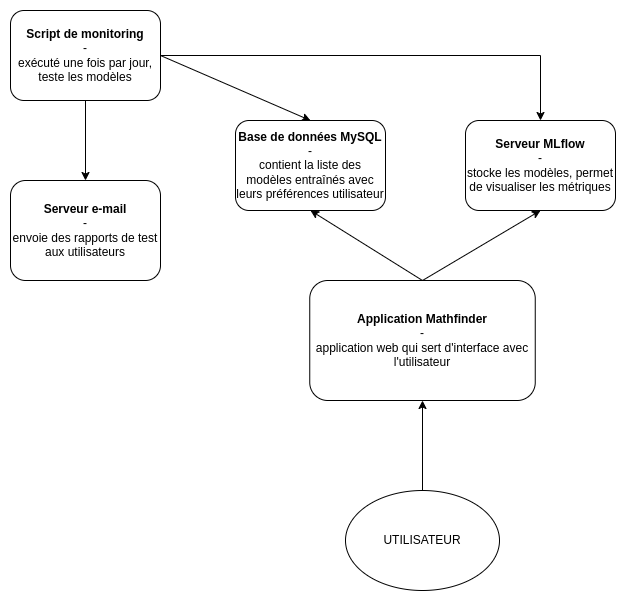
\includegraphics[width=8cm]{monitoring_E5}
        \centering
        \caption{Architecture de Mathfinder après avoir intégré un système de monitoring des modèles. Les flèches indiquent une relation d'usage (l'entité à l'origine de la flèche "utilise" celle vers laquelle la flèche se dirige)}
        \centering
    \end{figure}
    \subsection{Mise en place}
    Voici la procédure à suivre pour installer Mathfinder sur un serveur. Nous partirons ici du principe que Python et pip sont déjà installés.
    \begin{itemize}
        \item Pour commencer, récupérez le code de Mathfinder sur son dépôt GitHub. Vous pouvez le cloner, ou télécharger une archive qui contient tous les fichiers.
        \item Ouvrez un terminal dans le dossier où se trouve le code, et exécutez les commandes suivantes :
        \begin{verbatim}
            pip install pipenv
            pipenv install .
        \end{verbatim}
        \item Vous pouvez ensuite installer MySQL :
        \begin{verbatim}
            sudo apt update
            sudo apt install mysql-server
        \end{verbatim}
        Si votre serveur utilise Windows, \href{https://dev.mysql.com/doc/refman/8.3/en/windows-installation.html}{téléchargez l'installeur de MySQL} à la place. Lorsque MySQL est installé, créez une base de données puis exécutez cette commande :
        \begin{verbatim}
            mysql votre_bdd < mysql_dump.sql
        \end{verbatim}
        Ceci créera dans votre base de données une table Models dont Mathfinder aura besoin pour fonctionner.
        \item Exécutez ces commandes :
        \begin{verbatim}
            export MYSQL_USER="<votre nom d'utilisateur sur MySQL>"
            export MYSQL_PWD="<votre mot de passe sur MySQL>"
            export MYSQL_DB_NAME="<le nom de la base de données que vous avez créée sur MySQL>"
        \end{verbatim}
        \item Vous devez maintenant enregistrer le serveur que vous souhaitez utiliser pour gérer l'envoi d'e-mail (Google propose notamment ce service). Exécutez les commandes suivantes :
        \begin{verbatim}
            export SMTP_SERVER="<l'adresse de votre serveur SMTP>"
            export SMTP_LOGIN="<votre login sur ce serveur>"
            export SMTP_PWD="<votre mot de passe>"
        \end{verbatim}
        \item Enfin, vous pouvez lancer Mathfinder, le serveur MLflow et le script de monitoring. Exécutez ces trois commandes, dans l'ordre et chacune dans un terminal différent:
        \begin{verbatim}
            pipenv run mlflow server --host 127.0.0.1 --port 8080
            pipenv run streamlit run Mathfinder.py
            pipenv run python monitoring.py
        \end{verbatim} 
    \end{itemize}
    Mathfinder est maintenant opérationnel sur votre serveur !
    \section{Conclusion}
    Dans ce dossier, nous avons vu comment résoudre les bugs d'une application tout en utilisant la CI/CD pour protéger la qualité du code. Nous avons également vu comment mettre en place un système de suivi et d'alerte qui permet à de multiples utilisateurs de suivre l'évolution de leurs modèles d'IA. La structure présentée dans ce dossier est améliorable. On pourra ainsi envisager de créer son propre serveur SMTP ou encore d'exécuter MLFlow sur un serveur dédié.
\end{document}